\chapter{Interacción Débil}\label{cap:weak_int}
El origen de cada interacción fundamental se debe a causas diferentes. Por un lado, la existencia de carga eléctrica produce fuerzas electromagnéticas en las partículas y las hace interactuar entre sí, mientras que la interacción fuerte se debe a la propiedad del color, mencionada en el capítulo anterior. No todas las partículas tienen carga ni color simultáneamente por lo que no todas son susceptibles a las mismas interacciones. El caso de la interacción débil es bastante interesante porque muchas partículas con propiedades distintas son sensibles a ella. Por ejemplo, los leptones no tienen carga de color, no ``sienten'' la interacción fuerte; pero los neutrinos no tienen carga eléctrica por lo que no pueden interactuar mediante fuerzas electromagnéticas. Sin embargo, ambos tipos de partículas pueden estar presentes en interacciones débiles.\cite{Griffiths2008} Además, la causa de la interacción débil, aunque no tiene un nombre específico, suele denotarse como \textit{carga débil}.

Los mesones $K$ y muchas otras partículas decaen por interacción débil. Desde el principio se consideró un tratamiento cuántico-relativista para describir la interacción débil y muchos científicos han contribuido al desarrollo de su formalismo. Cada interacción ocurre gracias al intercambio de una partícula mediadora o portadora de la fuerza de interacción. En la interacción fuerte es el gluón y en la electromagnética es el fotón. Las partículas mediadoras encargadas de transmitir la fuerza débil entre los quarks y leptones son los bosones vectoriales, llamados así por tener espín 1. Estos bosones, de gran masa, portadores de la interacción débil pueden estar cargados eléctricamente $W^{\pm}$ o ser neutros $Z^0$. 

Hasta la década de los 70, sólo se habían observado procesos de intercambio de bosones cargados $W^{\pm}$. En los años 60 se empezó a formular una teoría que aunaba la interacción débil junto con la electromagnética, conocida hoy en día como \textit{Teoría Electrodébil}. Esta teoría predecía la existencia del bosón neutro mediador de la fuerza débil y dicha hipótesis fue confirmada experimentalmente en 1973 \cite{BrianM}, con el hallazgo de $Z^0$.

Este capítulo se centra, principalmente, en la descripción de procesos de interacción débil con intercambio de bosones $W^{\pm}$ o procesos de in\textit{teracción débil de corriente cargada} y nos servirá como base para el estudio del decaimiento de mesones $K$ cargados.


\section{Formalismo de la Interacción Débil}\label{cap:formalism}
\subsection{Teoría Cuántica de Campos: Interacción V-A}\label{sec:QFT}
De acuerdo con la Teoría Cuántica de Campos (TCC), cada partícula lleva asociado un campo cuántico $\phi(x)$, $\psi(x)$ o $W_{\mu}(x)$, dependiente del espacio y del tiempo $x^{\mu}=(ct,\boldsymbol{\vec{x}})$\protect\footnotemark. Estos campos $\phi(x)$, $\psi(x)$ o $W_{\mu}(x)$ actúan como operadores encargados de aniquilar partículas o crear antipartículas de espín $0$, $1/2 $ y $1$, respectivamente \cite{notas2020}.

\footnotetext{Consultar el Apéndice \hyperref[cap:A]{A} para más información sobre la notación utilizada en este capítulo.}
 
Para describir la evolución espacio-temporal de dichos campos asociados a partículas se hace uso de la densidad lagrangiana $\mathcal{L}$. Para las distintas partículas y sin tener en cuenta la interacción, en el sistema natural de unidades ($c=\hbar =1$), $\mathcal{L}$ tiene las siguientes expresiones:
\begin{itemize}
\item Bosones de espín $0$, tales como los mesones $K$ o los piones:
\end{itemize}
\begin{equation}
\mathcal{L}=-\partial ^{\mu }\phi \left( x\right) ^{\ast }\partial_{\mu} \phi \left( x\right) -m^{2}\phi \left( x\right) ^{\ast }\phi \left( x\right)
\end{equation}
El campo $\phi(x)$ tiene carácter escalar y es responsable de (crear) aniquilar (anti)partículas con $J=0$. $\phi^{\ast}(x)$ es su campo conjugado y hace justo lo opuesto: crea partículas y aniquila antipartículas con $J=0$.
\begin{itemize}
\item Fermiones de espín $1/2$, como los leptones:
\end{itemize}
\begin{equation}
\mathcal{L}=-\overline{\psi }\left( x\right) \left( \slashed{\partial}+m\right) \psi \left( x\right)
\end{equation}
$\psi(x)$ tiene carácter de espinor y (crea) aniquila (anti)partículas con $J=1/2$. Su adjunto también hace lo contrario.
\begin{itemize}
\item Bosones de espín $1$, como son los fotones o los bosones vectoriales $W$:
\end{itemize}
\begin{equation}
\mathcal{L}=-\dfrac{1}{4}\left| \partial _{\mu }W^{\nu }\left( x\right) -\partial _{\nu }W^{\mu }\left( x\right) \right| ^{2}-\dfrac{1}{2}m^{2}\left| W^{\mu }\left( x\right) \right| ^{2}
\end{equation}
Por último, $W^{\mu}(x)$ posee carácter de cuadrivector y se encarga de crear antipartículas y aniquilar partículas con $J=1$, mientras que su conjugado hace, nuevamente, lo opuesto.

Del mismo modo, las interacciones se describen mediante unas constantes, denominadas \textit{contantes de acoplamiento}, y productos entre los campos cuánticos de las partículas que intervienen en el proceso. Como $\mathcal{L}$ debe ser un escalar, sólo se permiten combinaciones entre campos que resulten en invariantes de Lorentz \cite{notas2020}. Esto es posible, ya que la TCC, entiende las interacciones como un intercambio de partículas mediadoras, tal y como se mencionó anteriormente. En su libro \cite{Bettini}, Bettini lo explica con el siguiente ejemplo: se tiene una partícula $a$ que interactúa en el campo mediado por el bosón $V$; en el vacío, $a$ está continuamente emitiendo y absorbiendo este bosón, tal y como se muestra en \ref{fig:bettini1}. No obstante, si una partícula $b$ se encuentra cerca de $a$ y tiene su misma interacción, puede absorber un bosón $V$ que previamente haya sido emitido por $a$ (ver \ref{fig:bettini2}). Entonces, se puede afirmar que $a$ y $b$ interactúan entre sí intercambiando un bosón $V$, es decir, combinando sus campos cuánticos.
\begin{figure}[h]
\begin{subfigure}{.5\textwidth}
  \centering
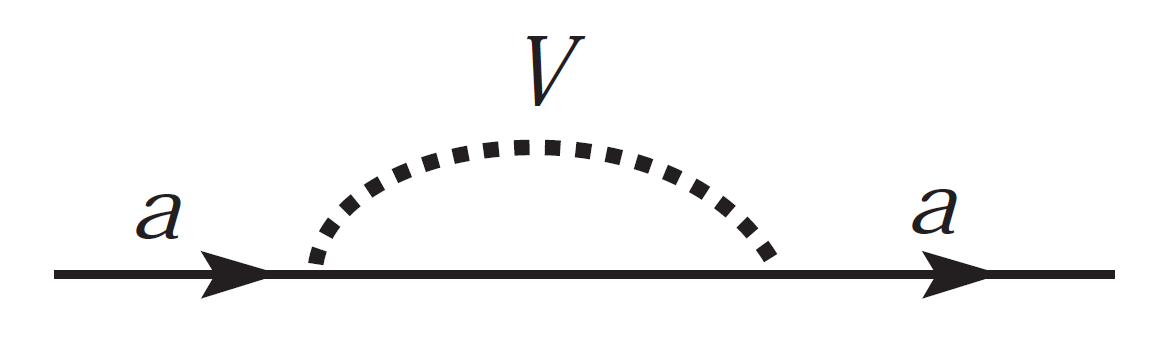
\includegraphics[width=0.6\linewidth]{{C:/Users/Carmen/Desktop/Universidad/TFG/Borradores/img/bettini1.PNG}}
\caption{$V$ emitido y reabsorbido por $a$}
  \label{fig:bettini1}
\end{subfigure}%
\begin{subfigure}{.5\textwidth}
  \centering
  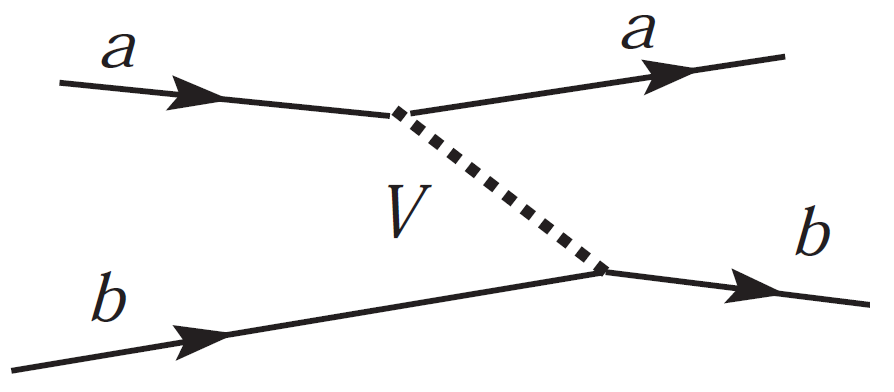
\includegraphics[width=0.6\linewidth]{{C:/Users/Carmen/Desktop/Universidad/TFG/Borradores/img/bettini2.PNG}}
  \caption{$V$ emitido por $a$ y absorbido por $b$}
  \label{fig:bettini2}
\end{subfigure}
\caption[Esquematización del proceso de interacción en TCC]{Proceso de interacción mediante intercambio del bosón mediador.  \cite{Bettini}}
\label{fig:bettini}
\end{figure}

Continuando con el ejemplo anterior, Bettini indica que el bosón mediador $V$ tiene, en general, una masa $m$ no nula, lo que provoca que, durante su emisión, se viole momentáneamente la conservación de energía $\Delta E = m$. Lo mismo, pero de forma opuesta ocurre durante su absorción. Así pues, la violación neta dura un $\Delta t$ y satisface la \textit{Relación de Indeterminación tiempo-energía}: $\Delta E \Delta t \leq \hbar$, lo que implica que $V$ sólo puede alejarse una distancia finita $R=c\Delta t$. Esta distancia equivale al rango de la fuerza de interacción, por lo tanto, cuanta mayor masa tenga el bosón mediador de una interacción, menor será su rango de alcance \cite{Bettini}. Dado que los bosones mediadores $W^{\pm}$ y $Z^0$ tienen una masa muy grande ($m_W=80,379 \pm 0,012$ GeV y $m_Z=91,1876 \pm 0,0021$ GeV, respectivamente \cite{Zyla}), la interacción débil tiene un alcance muy corto, más que cualquier otra interacción fundamental; de ahí la denominación de ``débil''. 

Gráficamente, las interacciones se representan con Diagramas de Feynmann. Estos diagramas proporcionan información acerca de la amplitud de probabilidad de los distintos procesos, donde cada línea representa a una partícula y cada vértice corresponde a cada actuación del lagrangiano de la interacción $\mathcal{L}$. Las líneas externas corresponden a partículas reales, mientras que las internas, que conectan los vértices, representan partículas virtuales, conocidas como propagadores o mediadores. El propagador es la partícula que se crea y aniquila; la que media la interacción. \cite{notas2020} En nuestro ejemplo anterior, dicho propagador sería el bosón $V$ y en el caso de la interacción débil, los propagadores serían los bosones vectoriales $W^{\pm}$ o $Z^0$.

La densidad lagrangiana $\mathcal{L}$ que describe cada vértice en el Diagrama de Feynmann de una Interacción de corriente cargada débil, tiene esta forma:
\begin{equation}
\mathcal{L}^{w}=\dfrac{g_{w}}{\sqrt{2}}\left( W^{\mu }\left( x\right) j_{\mu}^{+}\left( x\right) +\left[ W^{\mu }\left( x\right) \right]^{\ast }j_{\mu}^{-}\left( x\right) \right)\label{eq:weak_lagrangian}
\end{equation}
Recordemos que el campo $W^{\mu}(x)$ aniquila $W^{+}$ o crea $W^{-}$ mientras que su conjugado $\left(W^{\mu}(x)\right)^\ast$ aniquila $W^{-}$ o crea $W^{+}$. En un proceso que ocurre por interacción débil con intercambio de $W^{\pm}$, la carga neta del estado inicial y el final difieren en una unidad y, entonces, se habla de interacción de corriente cargada. Luego, la densidad de corriente débil $j_{\mu}$ puede ser positiva o negativa, y se compone de dos términos, uno para la corriente leptónica y otro para la hadrónica:
\begin{equation}
j_{\mu} ^{\pm }\left( x\right) =j_{\mu} ^{\pm lep}\left( x\right) +j_{\mu} ^{\pm had}\left( x\right) \label{eq:weak_current_hadylep}
\end{equation}
La corriente leptónica es una composición de corrientes de cada familia de leptones, así se tiene un término para los electrones, otro para los muones y otro para los taones:
\begin{equation}
j_{\mu }^{\pm lep}\left( x\right) =j_{\mu }^{\pm el}\left( x\right) +j_{\mu }^{\pm muon}\left( x\right) +j_{\mu} ^{\pm tau}\left( x\right)\label{eq:leptonic_weak_current}
\end{equation}
La corriente leptónica de electrones puede expresarse de la siguiente forma:
\begin{align}
j_{\mu }^{-el}\left(x\right)&=i\overline{\psi}_{e}\left( x\right) \dfrac{1-\gamma_{5}}{2}\gamma _{\mu }\psi_{{ \nu}_{e}}\left( x\right) & j_{\mu}^{+el}\left(x\right)&= i\overline{\psi}_{{\nu}_{e}}\left(x\right) \dfrac{1-\gamma_{5}}{2}\gamma _{\mu}\psi_{e}\left( x\right)\label{eq:electric_weak_current}
\end{align}
La corriente negativa $j_{\mu }^{-el}$, aniquila $\nu_e$ (o crea $\overline{\nu_e}$) y crea $e^-$ (o aniquila $e^+$), mientras que la corriente positiva $j_{\mu }^{+el}$ hace justo lo opuesto. $j_{\mu }^{\pm muon}$ y $j_{\mu }^{\pm tau}$ pueden definirse de manera análoga. Estas corrientes leptónicas se caracterizan por conservar el número cuántico leptónico y la carga de las partículas que intervienen. 

El operador de corriente hadrónica $j_{\mu} ^{\pm had}$ es el encargado de crear o aniquilar hadrones, conservando siempre el número bariónico $B$ e incrementando o reduciendo en una unidad la carga eléctrica total $Q$. Sin embargo, aunque no siempre, también son capaces de modificar la extrañeza: la corriente hadrónica positiva (negativa) puede aumentar (disminuir) la extrañeza en una unidad $\Delta S = +1$ ($\Delta S = -1$) \cite{notas2020}.

Además, $g_W$ es la constante de acoplo de la interacción débil y se relaciona con la constante de Fermi $G_F$ según \ref{eq:fermi_coupling}. Experimentalmente se ha comprobado que $G_F$ tiene un valor único para todos los procesos donde interviene la interacción débil, siendo este $G_{F}=1,166 \cdot 10^{-5}$ $GeV^{−2}$.
\begin{equation}
\dfrac{G_{F}}{g_{w}}=\dfrac{\sqrt{2}}{8m_{W}}\label{eq:fermi_coupling}
\end{equation}

Si se reescribe la corriente débil leptónica de la ecuación \ref{eq:electric_weak_current} en su forma expandida, pueden distinguirse dos términos:
\begin{equation}
j_{\mu}^{+el}\left(x\right)= \dfrac{i}{2} \{ \overline{\psi}_{{\nu}_{e}}\left(x\right)\gamma _{\mu}\psi_{e}\left( x\right)- \overline{\psi}_{{\nu}_{e}}\left(x\right)\gamma _{\mu}\gamma_{5}\psi_{e}\left( x\right) \}
\end{equation}
El primero $\overline{\psi}_{{\nu}_{e}}\gamma _{\mu}\psi_{e}$ se transforma como un vector polar (V) y el segundo término $\overline{\psi}_{{\nu}_{e}}\gamma _{\mu}\gamma_{5}\psi_{e}$ como un vector axial (A). Debido a esto, la corriente débil se dice que tiene estructura V-A. Esta estructura no es exclusiva para la corriente débil leptónica, sino que también está presente en la corriente débil hadrónica, salvo alguna constante de acoplamiento. 

Primeramente, se introdujo la parte correspondiente al vector polar en la corriente débil por analogía con la interacción electromagnética. El término del vector axial fue añadido posteriormente, tras el descubrimiento de la violación de paridad \cite{Paschos}. Si una interacción presenta la estructura anterior de Vector polar- Vector axial, se dice que es una \textit{Interacción V-A}.

Para describir los mesones $K$, como son partículas bosónicas de espín 0, se utiliza la ecuación Klein-Gordon. Esta ecuación tiene densidades de probabilidad negativas y, en general, es algo tedioso trabajar con ella. Debido a ello, es conveniente expresar los mesones $K$ según su composición de quarks (partículas fermiónicas) y así poder emplear la ecuación de Dirac, simplificando el estudio de las corrientes débiles.

Por lo tanto, el lagrangiano $\mathcal{L}$ de una interacción débil presentar estructura V-A o, en su forma más general, una combinación o producto de estructuras V-A \cite{Renton}, una para describir el decaimiento de los leptones y otra para los quarks:
\begin{equation}
\mathcal{L}= \sum _{i} C_{i}\left( \overline{\psi}_{\nu_l}\widehat{\Gamma_{i}}\psi _{l}\right)\left( \overline{\psi }_{q_2}\widehat{\Gamma^{i}}\psi _{q_1}\right)
\end{equation}
Los coeficientes $C_i$ son constantes de acoplamiento del proceso en cuestión y los $\psi_i$ son los bi-espinores resultantes de la ecuación de Dirac que describe cada fermión (quark o lepton) que participa en la interacción. Los $\widehat{\Gamma_{i}}$ son covariantes bilineales, los cuales proporcionan información sobre cómo se transforman las partículas que intervienen en el decaimiento (ver Apéndice \hyperref[cap:A]{A}).

\subsubsection{Helicidad y Quiralidad}\label{sec:quirality}

En las expresiones anteriores de la corriente débil leptónica aparece el operador $\gamma^5$, que indica la quiralidad de las partículas. A menudo, quiralidad y helicidad son conceptos confundidos. Por este motivo, es conveniente hacer un paréntesis y explicar con detalle en qué consiste cada uno.

La helicidad se define como la proyección del espín de una partícula en la dirección de su momento $\vec{p}$. En el marco teórico de la TCC, la helicidad de la partícula se representa mediante el operador helicidad $\mathcal{H}$:
\begin{equation}
\mathcal{H}=\dfrac{1}{2} \dfrac{\vec{p} \cdot \vec{s}}{p}
\end{equation} 

Para una partícula fermiónica (de espín $1/2$), los autovalores de $\mathcal{H}$ son $+1/2$, si la dirección de su espín coincide con la dirección de su movimiento, y $-1/2$ en el caso contrario \cite{Bettini}. Así pues, los autoestados de helicidad se corresponden a espinores de dos componentes. En general, si la partícula tiene una masa distinta de cero, la helicidad no es un invariante de Lorentz.

La quiralidad es una propiedad de los bi-espinores que se utilizan para definir partículas y se representa por los autoestados del operador $\gamma^5$, con valores propios $\pm 1$. Los estados de quiralidad son designados como positivo (R) y negativo (L), y sus proyectores son:
\begin{align}
\psi_L &= \dfrac{1-\gamma^5}{2}\psi & \psi_R &= \dfrac{1+\gamma^5}{2}\psi
\end{align}

El factor $\dfrac{1-\gamma^5}{2}$ es responsable de que sólo los leptones con quiralidad negativa reaccionen a la interacción débil y explica por qué, en esta interacción, pueden violarse P y CP, tal y como se detallará en el capítulo siguiente.

A diferencia de la helicidad, la quiralidad es siempre un invariante de Lorentz. Sin embargo, cuando la partícula fermiónica carece de masa, helicidad y quiralidad coinciden.

\subsection{Violación de Simetrías de Paridad y Carga}\label{sec:symmetry}
Antes de comenzar con la descripción de la teoría débil en el Modelo de Quarks, resulta adecuado tratar el tema de las simetrías para entender en mayor detalle el decaimiento de los mesones $K$ y el posterior capítulo de la violación CP.

Cuando ciertas propiedades de una partícula no cambian al someterla a un conjunto de transformaciones, se dice que esa partícula tiene una simetría. De acuerdo con el \textit{Teorema de Noether}, cada simetría se asocia a una magnitud física que se conserva, las cuales se describen mediante operadores hermíticos. Hay dos simetrías discretas importantes que conviene discutir en relación con los mesones $K$, ya que en la interacción fuerte y en la electromagnética se conservan, pero pueden violarse en la interacción débil. Estas dos simetrías son la inversión espacial P y la conjugación de carga C.

En la invariancia frente a la inversión espacial o simetría P (a veces, paridad $\pi$) se invierte el signo de las coordenadas de las partículas. En consecuencia, los vectores polares cambian su signo, como la posición $\vec{r}$ y el momento lineal $\vec{p}$, mientras que los vectores axiales, como el momento angular orbital $\vec{l}$, lo conservan. Esta simetría se describe mediante el operador paridad $\hat{P}$:
\begin{equation}
\begin{gathered}
\hat{P}\left| A;\vec{r};m\rangle =\eta_P\left(A\right) \right| A; -\vec{r}; m \rangle \\  \hat{P}| A; \Phi, l; m_{l}; m_{s} \rangle =\eta_P \left( A\right) \left( -1\right)^{l} | A;\Phi, l; m_{l}; m_s\rangle 
\end{gathered}
\end{equation}
La \textit{paridad intrínseca} $\eta_P(A)$ se determina empíricamente y se asocia con la estructura interna de la partícula A, pudiendo ser sus valores $\pm 1$. Para fermiones y bosones se tiene $\eta_P(f)=-\eta_P \left(\overline{f}\right)$ y $\eta_P(b)=\eta_P \left(\overline{b}\right)$, respectivamente. Además, se cumple que $[\hat{P}, \widehat{H}]=0$.

%\hat{P}\left| A; \vec{p}; \mathcal{H} \rangle =\eta_{P} \left(A\right) \right| A; -\vec{p}; -\mathcal{H} \rangle \\

De forma similar, la invariancia frente a la conjugación de carga o simetría C, transforma partículas $A$ en antipartículas $\overline{A}$ y viceversa, de modo que cambia el signo de la carga y del resto de números cuánticos aditivos $B$, $B$, leptónico $L$, etc. El operador asociado es $\hat{C}$:
\begin{equation}
\begin{gathered}
\hat{C}\left| A;\vec{p};s\rangle =\eta_C\left(A\right) \right| \overline{A}; -\vec{p}; s \rangle \\ \hat{C}| A; \Phi, l; m_{l}; m_{s} \rangle =\eta_C \left( A\right) | \overline{A};\Phi, l; m_{l}; m_s\rangle 
\end{gathered}
\end{equation}
De igual modo, $\eta_C(A)=\pm 1$ y $[\hat{C}, \widehat{H}]=0$. En este caso, sólo las partículas neutras tienen la \textit{paridad-C} $\eta_C(A)$ bien definida.
Estas dos simetrías parecían conservarse siempre en los procesos donde intervenían interacciones fundamentales.

\subsubsection{Enigma $\tau$-$\theta$}
Tras las primeras observaciones de los mesones $K$ en los años 50, había un par decaimientos de estas, por entonces llamadas, partículas $V$ que desconcertaba a los científicos de la época. Tanta era la confusión que incluso se llegó a pensar que había dos tipos de partículas $V$, a las que denominaron $\tau$ y $\theta$, como se mencionó en el capítulo anterior. 

Por una parte, en la fotografía \ref{fig:nature1}, se observaba el decaimiento $\theta^{0} \rightarrow \pi^{+}\pi^{-}$ y años más tarde también se había constatado la existencia del proceso $\theta^{+} \rightarrow \pi^{+}\pi^{0}$. Por otro lado, la fotografía \ref{fig:powell} mostraba la desintegración de $\tau^+ \rightarrow \pi^{+}\pi^{+}\pi^{-}$.  El estudio de estos dos procesos concluía que las partículas tau y theta eran idénticas pues tenían las mismas masas, las mismas vidas medias, etc., pero dado que los decaimientos tenían distinta paridad, era \textit{imposible} que fueran las mismas partículas; no se concebía que la paridad fuera violada. Esto hecho fue conocido como el \textit{enigma $\tau$-$\theta$} \cite{Ferbel}.
\begin{equation}
\begin{gathered}
\theta^{+} \rightarrow \pi^{+}\pi^{0} \Rightarrow \eta\left(\pi^{+}\right) \eta\left(\pi^{+}\right) = 1 \\ 
\tau^{+} \rightarrow \pi^{+}\pi^{+}\pi^{-} \Rightarrow \eta\left(\pi^{+}\right) \eta\left(\pi^{+}\right) \eta\left(\pi^{-}\right) = -1
\end{gathered}
\end{equation}

Tsung-Dao Lee y Chen-Ning Yang estudiaron a fondo el rompecabezas y concluyeron que no había ninguna evidencia para afirmar que la paridad se conservara en la interacción débil, por lo que las partículas $\tau$ y $\theta$ debían ser la misma y la violación de la paridad en esta interacción era una realidad más que plausible. 

El experimento clave que corroboró esta hipótesis,  realizado por Chien-Shiung Wu y Ernest Ambler, consistió en analizar la emisión $\beta$ del $\tensor*[^{60}]{\mathrm{Co}}{}$ polarizado,



\subsection{Interacción débil en el Modelo de Quarks}\label{sec:weak_int_quarks}
En el modelo de Quarks, la interacción débil se describe también mediante Diagramas de Feynmann pero esta vez se representa por medio de un cambio de sabor en los quarks, emitiendo a su vez bosones $W^{\pm}$. Según si un proceso de interacción débil, modifica o no su extrañeza, la expresión de corriente hadrónica puede variar:
\begin{itemize}
\item Si no cambia la extrañeza: se aniquila un quark $d$ y se crea un quark $u$.
\end{itemize}
\begin{equation}
j_{\mu}^{+had}(\Delta S= 0)=\cos \left( \theta _{c}\right) i\overline{\psi }_{u}\left( x\right) \dfrac{1-\gamma _{5}}{2}\gamma _{\mu }\psi _{d}
\end{equation}
\begin{itemize}
\item Si se modifica la extrañeza: se aniquila un quark $s$ y se crea un quark $u$.
\end{itemize}
\begin{equation}
j_{\mu}^{+had}(\Delta S= 0)=\sin \left( \theta _{c}\right) i\overline{\psi }_{u}\left( x\right) \dfrac{1-\gamma _{5}}{2}\gamma _{\mu }\psi _{s}
\end{equation}

En la interacción débil, el sabor $u$, de carga $+2/3$, se conecta con los otros dos sabores ligeros mediante $d\cdot \cos \left( \theta _{c}\right) +s\cdot \sin \left( \theta _{c}\right)$, donde $\theta _{c}$ hace referencia al ángulo de Cabbibo, cuyo valor experimental ha resultado ser $13,02\degree$. Del mismo modo, Cabbibo planteó que debería haber otro quark con la misma carga que $u$ pero que se conectara con la combinación ortogonal $-d\cdot \sin \left( \theta _{c}\right) +s\cdot \cos \left( \theta c\right)$, prediciendo así la existencia del quark pesado $c$.

Posteriormente, se concluyó que, en la interacción débil, todos los sabores de quarks, pesados y ligeros, debían estar conectados mediante la \textit{matriz CKM} (Cabibbo-Kobayashi-Maskawa). La importancia de esta matriz recae en sus términos diagonales, conectando: $u\leftrightarrow d$, $c\leftrightarrow s$ y $t\leftrightarrow b$. Los términos no diagonales son los responsables de que los quarks pesados vayan decayendo progresivamente en los sabores ligeros $u$ y $d$, que son los constituyentes predominantes de la materia ordinaria. La expresión de la matriz CKM es:
\begin{align}
d' &= V_{ud}\cdot d+V_{us}\cdot s + V_{ub}\cdot b \nonumber \\
s' &= V_{cd}\cdot d+V_{cs}\cdot s + V_{cb}\cdot b \label{eq:CKM}\\
b' &= V_{td}\cdot d+V_{ts}\cdot s + V_{tb}\cdot b \nonumber
\end{align}

Explicar de forma más ordenada


\section{Decaimiento de mesones $K$ cargados}
\label{sec:charged_kaon_decay}
Los mesones $K^{\pm}$ decaen por interacción débil y sus procesos de decaimiento (modos) pueden clasificarse en varias categorías. A continuación presentamos los modos leptónicos, semileptónicos y hadrónicos, que son los más relevantes:

\begin{table}[!htb]
\begin{minipage}{.5\linewidth}
    \centering
\begin{tabular}{ c c } 
\toprule
\makecell{Mesón $K^{+}$}  &  Mesón $K^{-}$ \\
\midrule   
$e^{+}\nu_{e}$ & $e^{-} \overline{\nu_{e}}$ \\
$\mu^{+}\nu_{\mu}$ & $\mu^{-} \overline{\nu_{e}}$ \\
$\pi^{0} e^{+} \nu_{e}$ & $\pi^{0} e^{-} \overline{\nu_{e}}$ \\
$\pi^{0} \mu^{+}\nu_{\mu}$ & $\pi^{0} \mu^{-} \overline{\nu_{e}}$ \\
$\pi^{0}\pi^{0} e^{+}\nu_{e}$ & $\pi^{0}\pi^{0} e^{-} \overline{\nu_{e}}$ \\
$\pi^{+}\pi^{-} e^{+}\nu_{e}$ & $\pi^{+}\pi^{-} e^{-} \overline{\nu_{e}}$ \\
$\pi^{+}\pi^{-} \mu^{+}\nu_{\mu}$ & $\pi^{+}\pi^{-} \mu^{-} \overline{\nu_{e}}$ \\
$\pi^{0}\pi^{0}\pi^{0} e^{+}\nu_{e}$ & $\pi^{0}\pi^{0}\pi^{0} e^{-} \overline{\nu_{e}}$ \\
\bottomrule
\end{tabular}
\caption[Modos de decaimiento leptónicos y semileptónicos de $K^{\pm}$]{Modos (semi-)leptónicos. \cite{Zyla}}
\label{tab:Kpm_leptonic_decay}
\end{minipage}\hfill
\begin{minipage}{.5\linewidth}
    \centering
\begin{tabular}{ c c } 
    \toprule
    \makecell{Mesón $K^{+}$}  &  Mesón $K^{-}$ \\    
    \midrule
$\pi^{+}\pi^{0}$ & $\pi^{-}\pi^{0}$ \\
$\pi^{+}\pi^{0}\pi^{0}$ & $\pi^{-}\pi^{0}\pi^{0}$ \\
$\pi^{+}\pi^{+}\pi^{-}$ & $\pi^{+}\pi^{-}\pi^{-}$ \\
    \bottomrule
\end{tabular}
\caption[Modos de decaimiento hadrónicos de $K^{\pm}$]{Modos hadrónicos. \cite{Zyla}}
\label{tab:Kpm_hadronic_decay}
\end{minipage}
\end{table}

Como puede observarse, los modos de decaimiento de $K^{-}$ son los mismos modos que los de $K^{+}$ pero con carga conjugada. Sin embargo, no todos estos procesos tienen la misma probabilidad de ocurrir. ¿A qué se debe esto y cuáles son los factores que determinan esta probabilidad?. Para responder a estas preguntas nos centramos en el estudio de los modos leptónicos del kaón positivo: $K^{+} \rightarrow e^{+}\nu_{e}$ y $K^{+} \rightarrow \mu^{+}\nu_{e}$.

Para calcular la probabilidad de decaimiento de los mesones $K$ hacemos uso de la siguiente expresión:

VER GRIFFITHS, CAPITULO 10: WEAK INTERACTIONS - PION DECAY